\tightsection{Background and Motivation}

\jc{the following paras are directly moved here from old version of intro. need to be better organized!}
How are protocols designed?  To somewhat oversimplify: The designer implicitly or explicitly builds a model of the world, from which predictions about outcomes of decisions are made.  Then the protocol takes the decision that optimizes the utility of the predicted outcome.  For example, if it were possible to perfectly predict whether packet loss would occur given a particular TCP initial window size, we could maximize the QoS and user experience by choosing the highest initial window size that wouldn't cause a packet loss.  Similarly, if we could perfectly predict whether a client could sustain a particular bitrate, we could choose the highest sustainable bitrate.

Of course, modeling the world is difficult, and often we must use information from the real world to inform our models.  When is data-driven modeling important?  Generically, using data is helpful if our decisions are important (since otherwise we don't stand to gain much through better modeling) and the world is complex enough that we cannot model it well otherwise \henry{how complex? and why such complexity makes model insufficient?}.

We argue that protocol design is no different: We can accurately predict the outcomes of protocol decisions by sharing the clients' information. The main idea is to use the performance of existing clients to predict the performance of another client. For example, when a new client starts streaming a video, we can use the quality experienced by other clients to predict the quality that would be experienced by the new client when streaming at a given bitrate. Based on this prediction, we can then select the optimal bitrate for the new client.  In TCP protocol design, we might gather data about many TCP connections to discover the distribution of packet loss rates for different initial window sizes.  \jc{Also cite sigcomm'12 paper on data-driven TCP design which argues that TCP parameters need to be driven by real data}

We refer to the resulting model\henry{need a different word for this; ``model'' is now unfortunately overloaded} of sharing information across clients and making decisions based on predictions made by shared information as a predictive decision model. We note that predictive decision model which requires sharing the information across clients at a global scale is naturally enabled by today's service architectures where a very large number of clients are typically connected to a backend at any given time. Google, Facebook, Microsoft, Yahoo!, and Twitter are just a handful of sites that can observe the quality and the performance experienced by a huge number users at any give time. Thus, maximizing the QoS of existing applications using predictive decision model does not require new architectures or building new large scale systems; it can be done in the context of the already existing artifacts.  However, due to the complexity of networks -- in particular their temporal and spatial heterogeneity -- we find it is necessary to bring a degree of statistical sophistication to network modeling algorithms.

In this paper, we apply the idea of predictive decision model to video quality optimization in the context of a large site that manages the video delivery of many premium content brands such as HBO, MOL, and ESPN. Video traffic is singularly important as it dominates the Internet traffic today, and this domination will only intensify in the forseable future. We describe a solution architecture, called Video Global Optimization (GO) and the associated algorithms to collect and use real-time quality-related information from every client currently streaming video to predict the quality of another user if she were streaming from a particular CDN at a particular bittrate, and use this prediction to select initial bit rate and CDN for a new user.

\ion{... something on how this is cross-layer SDN...}

\jc{need a better transition from the general idea of prediction-centric to video-specific optimization.}

\tightsubsection{Need of quality prediction}

\myparasum{Today's video quality} Previous research has confirmed the impact of quality on user experience that users are quite sensitive to buffering and high startup latency, and prefer higher bitrate content. Moreover, it also has been confirmed that today's end user experience is far from perfect and quality optimization is needed\cite{sigcomm12,conext13}.

\myparasum{What decisions can be made for a video session} A typical way of Internet video delivery is that during a video session, the video player streams the video object from a server by sequentially downloading chunks in a progressive of periodical fashion. Today's video delivery infrastructure provides two control knobs -- {\it CDN} in which the server is located, {\it bitrate} in which the object is encoded -- for a video player to adapt against changes in network condition and resource availability. The CDN and bitrate can be chosen from a pre-determined set of options and can be switched at any point during a session. For instance, to play a video that is encoded in $n$ levels of bitrates and stored on $m$ CDNs, a video player can start with or switch to use any CDN with any bitrate among the $m\times n$ options.
Readers may refer to~\cite{conext12} for more details. 

\myparasum{Previous research has shown prediction is necessary} In this context, video quality can be optimized by making the best decision (i.e., CDN, bitrate) for each session. Previous research \cite{sigcomm12,conext13} has provided insights on the potential of such optimization. In particular, it has shown (1) significant spatial diversity in CDN performance \footnote{CDN performance means the overall video quality that viewers experience if the video is streamed from it.} and availability across different geographical regions and ISPs; (2) substantial temporal variability in the CDN performance and client-side network performance; and (3) that causes of quality issues can be rooted in various attributes of a session (e.g., content provider, player implementation, or a combination). These results imply that there is no globally best decision which performs better than others for most sessions (in space) and for most of time (in time), and therefore, the best decision for any session should be made by predicting the video quality of each decision if it were to be used. 

\tightsubsection{Need of using client measurement}
\jc{this subsection is logically needed, but not easy to argue.}

In order to accurately predict the outcome of each decision, one approach is to have static models that characterize the quality of each decisions. However, this approach can be highly (1) complex as there are many entities that affect the quality along the path from video source to client in today's video delivery infrastructure~\cite{?}, and (2) costly to maintain as each session's quality may be affected by any factor. Alternatively\footnote{As also argued in~\cite{sigcomm13DataDrivenTcp}}, we argue that by continuously collecting information about the performance of existing sessions, we will be able to predict the quality of new video sessions by looking at the performance of existing sessions that are close to it.



\tightsubsection{Dataset}
\label{subsec:dataset}

\myparasum{Dataset overview} To motivate the use of client measurement information and examine our techniques, we use a dataset of client-side quality measurement. Our dataset is based on client-side measurements of video quality from over \fillme million sessions or views (both successful and failed) over a duration of \fillme days. The data was generated via client-side player instrumentation that monitors the state of player and network condition, collects the statistics regarding the observed video quality (e.g., rebuffering ratio, chosen bitrate) and session attributes (e.g., ASN, chosen CDN, player type). These collected information will be sent back to the backend so that we can maintain up-to-date quality and attribute information of each observed session.

\myparatight{Quality sample} The basic unit in our dataset is a {\it quality sample}\jc{quality sample is just more expressive way of SessionInterval.}. A quality sample represents a user viewing a video on one of our affiliates' sites for a fixed interval of time\jc{is SessionInterval always for one minute in current implementation?}. Each quality sample is associated with four fields -- session ID, attributes, timestamp and quality metrics. 

\myparatight{Attributes} There are \fillme attributes that we observe and collect at client-side:

\begin{packedenumerate}
\item \emph{ASN:} The Autonomous System Number (ASN) that the client IP belongs
 to. Note that a single ISP (e.g., Comcast) may own different ASNs both
 for management and business reasons. We focus on the ASN as it is more fine-grained
 than the ISP granularity.  We observe in aggregate \fillme unique ASNs
  spanning multiple countries.

\item \emph{Object:} The object is an unique ID for each video object. We observe in aggregate \fillme objects.

\item \emph{Content provider (Site):} This is the specific affiliate content
provider from which the client requested some content. We have  \fillme content
providers that span different genres of content.  We use the terms site and
content provide interchangeably.

\item \emph{Initial CDN:} This is the CDN that the video session starts with.  In total, we observe
\fillme unique CDNs spanning popular CDN providers as well as several in-house and
ISP-run CDNs. (Some providers use proprietary CDN switching logic; in
this case we pick the segment of the session with the CDN used for the longest
duration.)

\item \emph{Initial Bitrate:} This is the bitrate that the video session starts with. The set from which the initial bitrate is chosen depends on the encoding of each video. \fillme of the video objects we observe have multiple bitrates.

\item \emph{OS:} In many cases, the OS of client device on which the video is played determines the streaming protocol of player type. For example, when watching the same video, iOS clients use different player than other OSes.

\item \emph{Connection type:} Finally, we  have the type of
access network connection such  as
 mobile/fixed wireless, DSL, fiber-to-home. These annotations come from third party services~\cite{quova}.

Notice that initial decision (i.e., initial CDN and initial bitrate) is also counted as attributes in quality samples.

\end{packedenumerate}

\myparatight{Quality metrics} We focus on four industry-standard video quality metrics that have been shown to be critical for measuring user engagement~\cite{sigcomm11}. They reflects the video quality during a fixed time window (e.g., 1 minute).
\begin{packedenumerate}
\item \emph{Buffering ratio:}  Given a video session of duration $T$~seconds,
if the player spent $B$~seconds in buffering (i.e., waiting for the player
 buffer to replenish midstream, the buffering ratio is defined as
 $\frac{B}{T}$. Prior work has shown that buffering ratio is a key metric
 that impacts user engagement~\cite{sigcomm11}.
\item \emph{Join time:}  This is the time taken for the video to start playing
 from the time the user clicks on the ``play'' button on the player.
 While join time may not directly impact the amount of a specific video viewed,
 it does have long term effects as it reduces the likelihood of repeated
visits~\cite{sigcomm11,akamai-imc12}. 
\item \emph{Average bitrate:} Many video players today support adaptive bitrate
selection and midstream bitrate switching to adapt to changing bandwidth
availability. The average bitrate of a session is simply the time-weighted
average of the bitrates used in a given session. (Bitrate refers to the video playback rate, rather than throughput or download rate.)
\item \emph{Start failures:}   Some sessions may not even start playing the
video; either the content is not available on the CDN server or the CDN is
under overload or other unknown reasons. We mark as a session as a join failure
if no content was played during this session.\footnote{Start failures are
reported by the client-side measurement module that sends a ``heartbeat'' on
the player status.}
\end{packedenumerate}
Join time and start failures are valid metrics only for those sessions that just join the session.

\myparatight{Timestamp} The timestamp is the system at backend when the sample is received from client. There are two sources of measurement noise in our implementation: (1) The backend system time is different from when the sample is actually collected. (2) Some quality metrics (e.g., join time) reflect the quality at the beginning of a session of rather than the current time point. \jc{The impact of each of these noise should be discussed later.}

\tightsection{GO system overview}
\label{sec:overview}

\myparasum{We have built a real system} The richness of our dataset allows us to make more informed decisions. We have implemented a working prototype called Video Global Optimization (GO) to realize this goal and to actually improve video quality in the wild.  Here we describe its architecture for gathering data, predicting quality and making decisions; the remainder of this paper will focus on the mapping from data to decisions via prediction.

\myparasum{Highlevel components} Physically, in order to collect statistics from client and make decision in a centralized manner, GO has two parts: instrumentation code running within client-side players during the cause of a video session, and the GO backend running in publicly available clusters for centralized processing. Logically, there are three following components of GO system (see Figure~\ref{fig:go-overview}). 

\myparatight{Quality sample collection} To collect feedback from client-side video sessions, the instrumentation code monitors the states of player and network condition, summarizes them in the form of quality samples (see details in \Section~\ref{subsec:dataset}) and send the quality samples back to the GO backend. The GO backend stores all quality samples in a Hadoop File System for storage and scalable access. \jc{in reality, the raw input from client is in log format of heartbeat, and later processed into quality samples by the backend. we may decide whether to expose it in scalability section.}

\begin{figure}[h!]
\centering
 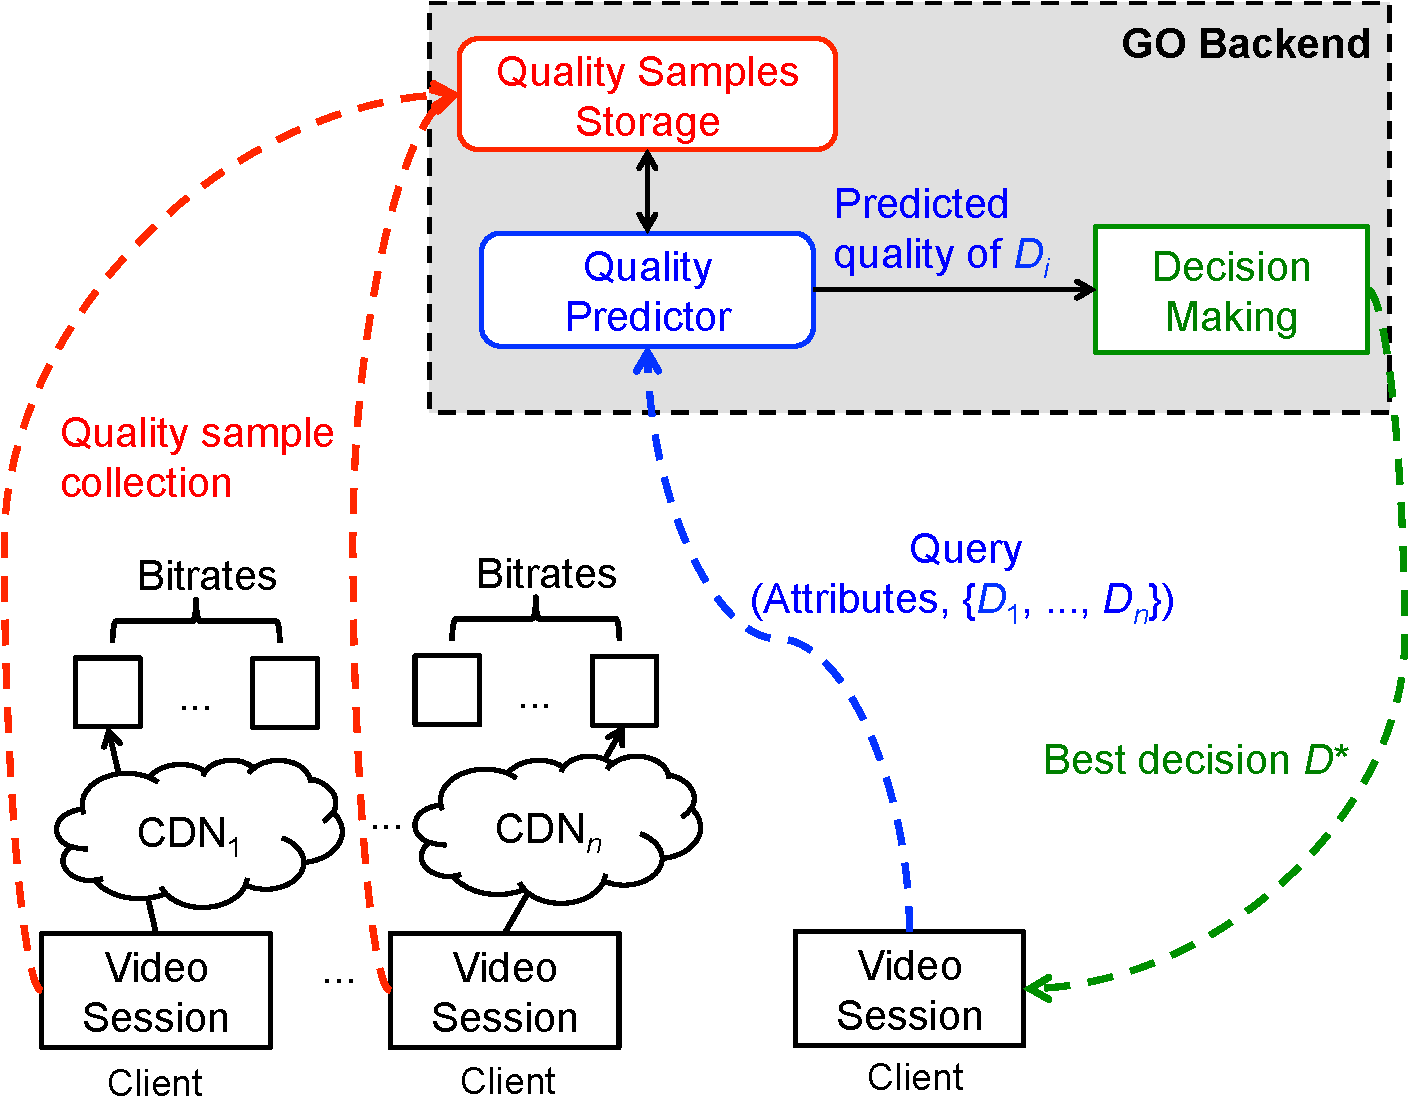
\includegraphics[width=0.5\textwidth] {figures/go-overview.pdf}
\tightcaption{Architecture of GO.}
\label{fig:go-overview}
\end{figure}

\myparatight{Quality prediction} Quality samples are mapped to predictions about quality outcomes of future sessions for each possible decision.  We postpone discussion of the details of this mapping for now.  For efficiency reasons, this step cannot rely on all available quality samples; they must be sampled or aggregated in some fashion.

\myparatight{Decision making} A simple procedure is used to decide on the optimal CDN or bitrate for a video session: A predicted quality metric is computed for each possible decision, and then the decision maximizing predicted quality is taken.  Since there are multiple quality metrics, they must be combined into a single figure of merit via a \emph{utility function}\jc{We do not really use the notion of utility function now. Remember to echo this point later on.}.  For example, a utility function may return a linear combination of several quality metrics.
